\section{Theorie}
\label{sec:Theorie}

Zunächst wird der prinzipielle Aufbau eines Sagnac-Interferometers erklärt.
Danach wird die Bedeutung von einigen wichtigen Variablen (Kontrast) erklärt.

\subsection{Das Sagnac-Interferometer} \label{sec:aufbau}

\begin{figure}[h]
    \centering
    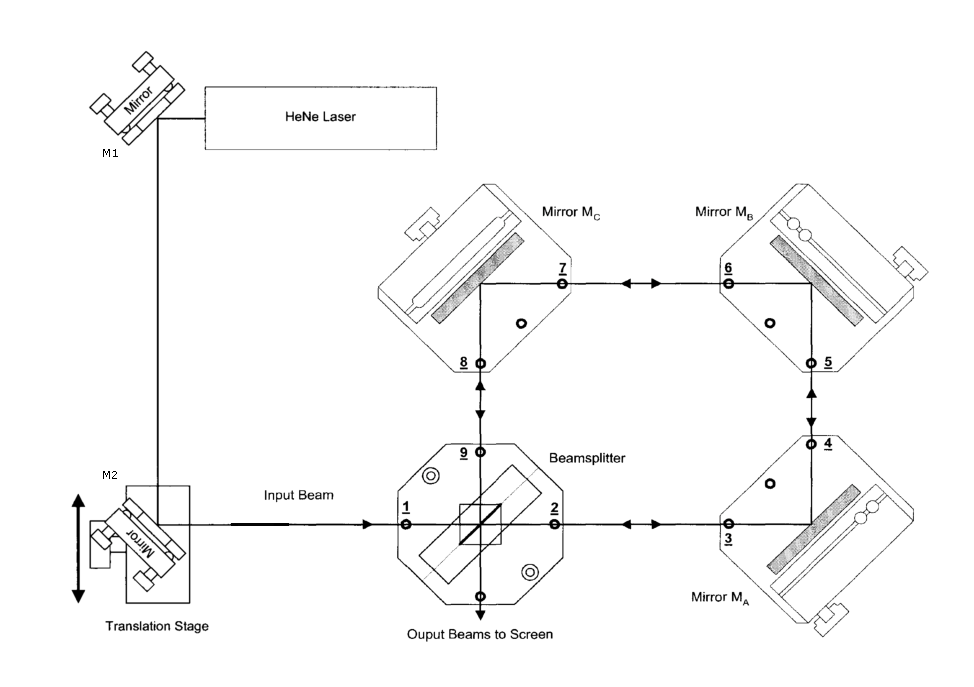
\includegraphics[width = 0.7 \linewidth]{pictures/aufbau1.pdf}
    \caption{Schematischer Aufbau eines Sagnac-Interferometers.\cite{v64}}
    \label{aufbau1}
\end{figure}

In \autoref{aufbau1} ist der grundlegende Aufbau eines Sagnac-Interferometers schematisch abgebildet.
Dieser besteht aus insgesamt 6 Spiegeln.
Dabei sind die Spiegel zur Strahljustierung vorgesehen.
M2 wird auch genutzt, um die beiden Strahlen voneinander zu trennen.
Dies geschieht dadurch, dass das Licht aus dem Helium-Neon-Laser so auf den PBSC (Polarizing-Beam-Splitter-Cube) gelenkt wird, dass der Strahl nicht mittig auftrifft.
Durch diese Verschiebung laufen die Strahlen zwar am Ende wieder (bei justierten Spiegeln) ineinander zusammen, lassen sich jedoch getrennt voneinander manipulieren, beispielsweise durch ein Glasplättchen.
Nachdem die Strahlen wieder zusammengeführt wurden, werden sie schließlich durch ein um 45°  gedrehten PBSC wieder getrennt und polarisiert und auf zwei verschiedene Photodioden gelenkt.
Dies passiert zu Gunsten der sogenannten Differenzspannungsmethode.
Bei Anwendung dieser Methode liegt der Vorteil darin, dass hinterher die beiden Signale voneinander abgezogen werden und somit äußere Störfaktoren wie Restlicht im Laborraum systematisch herausgerechnet werden können.
Unter anderem durch diese Methode ist das Sagnac-Interferometer nicht so störungsempfindlich wie andere Interferometer. 

\subsection{Kontrast} \label{sec:kontrast}
Als Kontrast (oder Sichtbarkeit) eines Interferometers wird die Beziehung
\begin{equation} \label{eq:kontrast}
    K = \frac{I_\text{max} - I_\text{min}}{I_\text{max} + I_\text{min}}
\end{equation}
bezeichnet. Offensichtlich gilt also für den Kontrast: $K \in [0,1]$.
Anschaulich beschreibt $K$ wie klar das Interferenzbild ist.
Bei einem Kontrast von $0$ wäre beispielsweise kein Interferenzbild messbar.

Für die Intensitätsmaxima/- und minima gilt die Beziehung \cite{v64}
\begin{equation*}
    I_\text{max/min} \propto I_\text{Laser} \left[ 1 \pm 2 \cos(\Phi) \sin (\Phi) \right] \, ,
\end{equation*}
aus der sich wiederrum mit \autoref{eq:kontrast} die Gleichung
\begin{equation*}
    K = K(\Phi) \propto \frac{\left[ 1 + 2 \cos(\Phi) \sin (\Phi) \right] - \left[ 1 - 2 \cos(\Phi) \sin (\Phi) \right]}{\left[ 1 + 2 \cos(\Phi) \sin (\Phi) \right] + \left[ 1 - 2 \cos(\Phi) \sin (\Phi) \right]}
    = 2 \cos(\Phi) \sin(\Phi)
\end{equation*}
ergibt. Hieraus ist auch sofort ersichtlich, dass der Kontrast bei ungefähr $45°$ am höchsten sein dürfte, wenn alle anderen Einflüsse optimiert sind.

\subsection{Brechungsindizes} \label{sec:n}

Der Brechungsindex eines Mediums ist eine intrinsische Eigenschaft eines Materials.
Diese sind auch mit einem Interferometer bestimmbar.
Es ist bekannt, dass ein Medium mit $n_\text{Medium} > 1$ die Geschwindigkeit von Licht verringert.
Dies lässt sich durch die Gleichung
\begin{equation*}
    v_\text{Vak} = \frac{c}{n}
\end{equation*}
beschreiben. Wird also ein Lichtstrahl durch ein Medium gelenkt, dabei reicht bereits eine geringe Strecke aus, erfährt dieser Lichtstrahl im Gegensatz zu einem anderen Lichtstrahl der selben Quelle eine Phasenverschiebung.
Dies lässt sich in Interferometern ausnutzen, um den Brechungsindex eines Mediums zu bestimmen.
Für die Phasenverschiebung in Luft gilt die Beziehung \cite{v64}
\begin{equation} \label{eq:nluft}
    \Delta \Phi = \frac{2 \pi}{\lambda_\text{vac}} \Delta n \cdot L \, ,
\end{equation}
dabei ist L die Länge der durchquerten evakuierten Zelle.
Wird nun die Beziehung der gezählten Intensitätsmaxima 
\begin{equation} \label{eq:maxima}
    M = \frac{\Delta \phi}{2 \pi}
  \end{equation}
in \autoref{eq:nluft} eingesetzt, lässt sich dieser durch die Gleichung
\begin{align}
    \Delta n &= n_\text{Medium} - n_\text{Vak} = \frac{M \cdot \lambda_\text{vac}}{L} \\
    n_\text{Medium} &= \frac{M \cdot \lambda_\text{vac}}{L} + 1
\end{align}
bestimmen.

In diesem Experiment wird auch durch zwei verkippte Glasplättchen der Brechungsindex von Glas bestimmt.
Für den Brechungsindex in Glas gilt allgemein \cite{v64}
\begin{equation}\label{eq:phiglas}
    \Delta \phi = \frac{2\pi}{\lambda}T\left(\frac{n-1}{2n}\Delta \theta^2+O( \Delta \theta^4)\right) \, .
\end{equation}
Diese Gleichung muss zunächst modifiziert werden, da 2 Glasplättchen verbaut sind und dazu um $\Theta_0 = \pm 10°$ verkippt sind.
Damit wird aus \autoref{eq:phiglas} die Gleichung in führender Ordnung
\begin{equation}
    \Delta \phi = \frac{\pi \cdot (n - 1) T}{\lambda \cdot n} \left(\left( \theta + 10° \right)^2 - \left( \theta - 10° \right)^2\right) \, ,
\end{equation}
was mit \autoref{eq:maxima} auf die Gleichung
\begin{equation*}
    M = \frac{n - 1}{\lambda \cdot n} \cdot \theta \cdot |\theta_0|
\end{equation*}
und somit auf
\begin{equation} \label{eq:n_Glas}
    n = \frac{1}{1- \frac{\lambda M}{ \theta \cdot |\theta_0| T}}
\end{equation}
führt.